\documentclass{jsarticle}
\usepackage[dvips]{graphicx}
\usepackage{fancyhdr}
\setcounter{page}{0}
\begin{document}

\title{制御工学実験II \\ 4.サーボモータの周波数同定}
\author{提出者 \\ 14104064 下松八重 宏太 \\ \\ 共同実験者 \\ 14101028 梶野 翔平 \\ 14104092 中島 美香 \\ 16104311 北山 拓夢 \\ 13104119 廣瀬 直人}
\date{提出日 2016年4月26日 \\ 再提出日 2016年5月10日 \\ 再々提出日 2016年5月24日}



\maketitle
\thispagestyle{empty}
\newpage

 \section{目的}
  サーボモータを対象とし,制御対象の未知パラメータを同定するための一つの手法を習得することを主目的とする.また,この同定実験を通し,対象を同定することがどのようなことなのかを理解する.
 
 \section{原理}
  \subsection{対象の数学モデル}
   \subsubsection{実験装置の概観}
    本実験で用いる実験装置の概要を図\ref{fig:souti}に示す.図\ref{fig:souti}の下部にある円盤がモータにより回転し,エンコーダで円盤の回転角度を検出する.計算機に取り込む際には角度[deg]を電圧[V]に変換した値を取り込む.

   \begin{figure}[bp]
    \begin{center}
     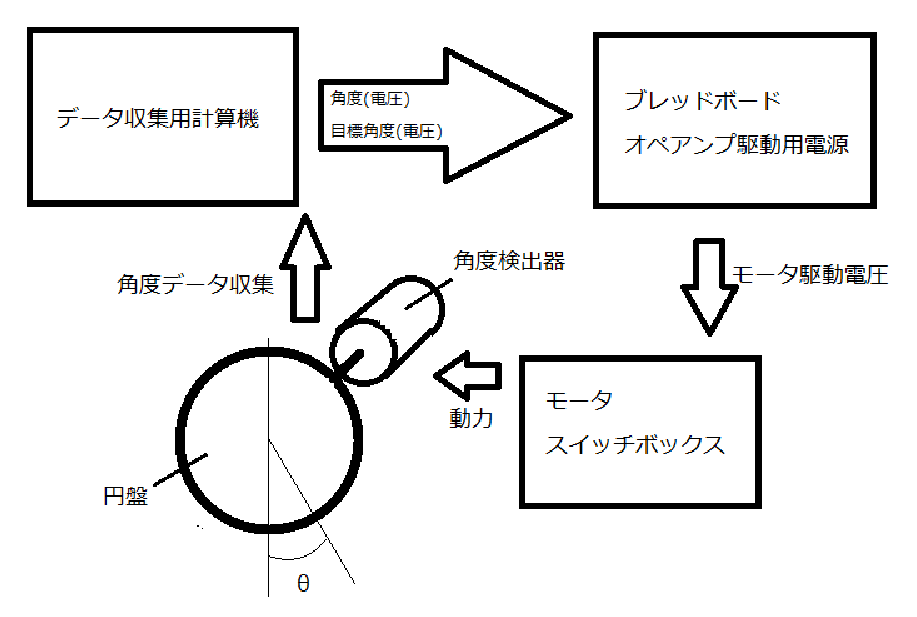
\includegraphics[scale=.5]{./picture/souti.eps}
     \caption{実験装置の概観}
     \label{fig:souti}
    \end{center}
   \end{figure}
   
   \subsubsection{モータの動特性}
 モータの特性を図\ref{fig:tokusei}に示す.
\begin{figure}[b]
 \begin{center}
  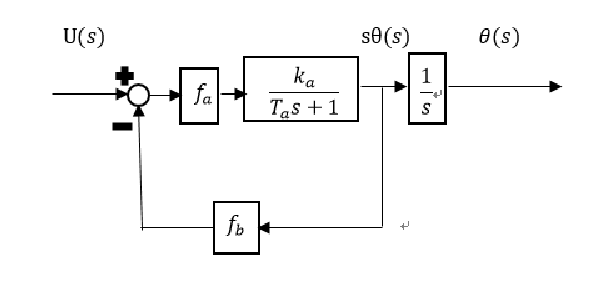
\includegraphics[scale=1]{./picture/blocks.eps}
  \caption{モータ特性}
  \label{fig:tokusei}
 \end{center}
\end{figure}

このとき,入力電圧から円盤角度までの特性は
\begin{equation} 
 \Theta(s) = \frac{1}{s}\,\frac{\frac{1}{f_b}}{\frac{T_a}{f_a f_b k_a}s + \frac{1}{f_a f_b k_a} + 1}U(s)
\end{equation}
となる.フィードバックゲイン$f_a$, $f_b$は
\begin{equation}
 0 < \frac{1}{f_a} << 1, f_b \simeq 1
\end{equation}
となるように設定してあるので,
\begin{equation}
 \frac{1}{s}\,\frac{\frac{1}{f_b}}{\frac{T_a}{f_a f_b k_a}s + \frac{1}{f_a f_b k_a} + 1}U(s) \simeq 1
  \label{eq3}
\end{equation}
となり,近似的に
\begin{equation}
 \Theta(s) = \frac{1}{s}U(s)
\end{equation}
と表現される.
\\本実験ではモータの入力電圧から円盤の回転角までの伝達特性は
\begin{equation}
 \label{eq5}
  \Theta(s) = \frac{k}{Ts + 1}U(s)
\end{equation}
で与えられる.{\it T}は時定数,{\it k}はゲインで,未知である.

   \subsection{周波数応答を用いた同定法}
   式\ref{eq5}で表現される制御対象に正弦波目標角度$u(t) = asin\omega_i t$を印加したとき,出力は
   \begin{equation}
    \label{eq6}
     \theta(t) = b_i e^{-\frac{1}{T}t} + c_i sin(\omega_i t + \phi_i)
   \end{equation}
   の形で表現される.式\ref{eq6}において$\phi_i$は位相を表す定数である.一般に時定数{\it T}は正の実数なので,十分時間がたてば,式\ref{eq6}の右辺第1項はほぼ0となり,
   \begin{equation}
    \theta(t) \simeq c_i sin(\omega_i t + \phi_i)
   \end{equation}
   となる.十分時間がたち,入力が0から正に増加するときの時刻を0とすると出力は正弦波となる.その振幅は目標角度振幅の$c_i / a$倍となる.また,入力が0から正に増加するときの時刻$t_i$は目標角度から$- \phi_i / \omega_i$秒ずれる.この振幅比$c_i / a$ならびに$\phi_i$のことを,周波数$\omega_i$に対する制御対象のゲインと位相と呼ぶ.種々の周波数に対するゲインと位相を片対数グラフにプロットしたものをボード線図を呼ぶ.\\
   式\ref{eq5}の時定数{\it T}とゲイン{\it k}が未知のときでも,ボード線図より低周波ゲイン\=kと折れ点周波数$\omega_d$[rad/s]の値がわかれば,
\begin{equation}
 \bar{k} = 20\log{10} k, \omega_d = \frac{1}{T}
  \label{eq8}
\end{equation}
の関係より制御対象の時定数とゲインを知ることが出来る.

 \section{実験方法}
 \begin{enumerate}
  \item 周波数同定実験用のプログラムを起動する.
  \item データ収集用サンプリング周期{\it h}を0.01[s]とし,学籍番号,目標角度周波数$\omega$を入力して測定を開始する.($\omega = 0.1 ~ 10$[rad/s]の範囲で測定する.必要なら10[rad/s]以上の周波数に対する測定を行ってもよい.)
  \item 収集した実験データよりゲイン,位相を計算し,片対数グラフを用いてボード線図をプロットする.
  \item ボード線図より,対象の時定数{\it T}とゲイン{\it k}を求める.
 \end{enumerate}
 
\section{実験結果}
測定結果を表\ref{tab:table1}に示し,得られたボード線図を図\ref{fig:board}に示す.\\
\begin{table}[hb]
 \begin{center}
  \caption{測定結果}
  \begin{tabular}{|c|c|c|} \hline
   目標角度周波数 & ゲイン{\it k}[dB] & 位相$\phi_i$[deg]\\ \hline \hline
   0.1 & 0 & 0 \\ \hline
   0.2 & 0 & -4.56 \\ \hline
   0.4 & 0 & -6.88 \\ \hline
   0.6 & -0.14 & -10.4 \\ \hline
   0.8 & -0.32 & -15.4 \\ \hline
   1.0 & -0.39 & -16.6 \\ \hline
   2.0 & -1.27 & -31.4 \\ \hline
   2.4 & -1.72 & -38.2 \\ \hline
   2.6 & -1.94 & -41.5 \\ \hline
   2.8 & -1.94 & -43.4 \\ \hline
   2.9 & -2.85 & -45.3 \\ \hline
   3.0 & -2.95 & -46.1 \\ \hline
   3.2 & -2.85 & -47.0 \\ \hline
   3.4 & -2.85 & -49.5 \\ \hline
   4.0 & -4.44 & -55.9 \\ \hline
   5.0 & -5.68 & -60.1 \\ \hline
   6.0 & -6.38 & -65.6 \\ \hline
   8.0 & -8.87 & -75.2 \\ \hline
   10.0 & -10.0 & -82.6 \\ \hline
  \end{tabular}
  \label{tab:table1}
 \end{center}
\end{table}

\newpage

\begin{figure}[hb]
 \begin{center}
  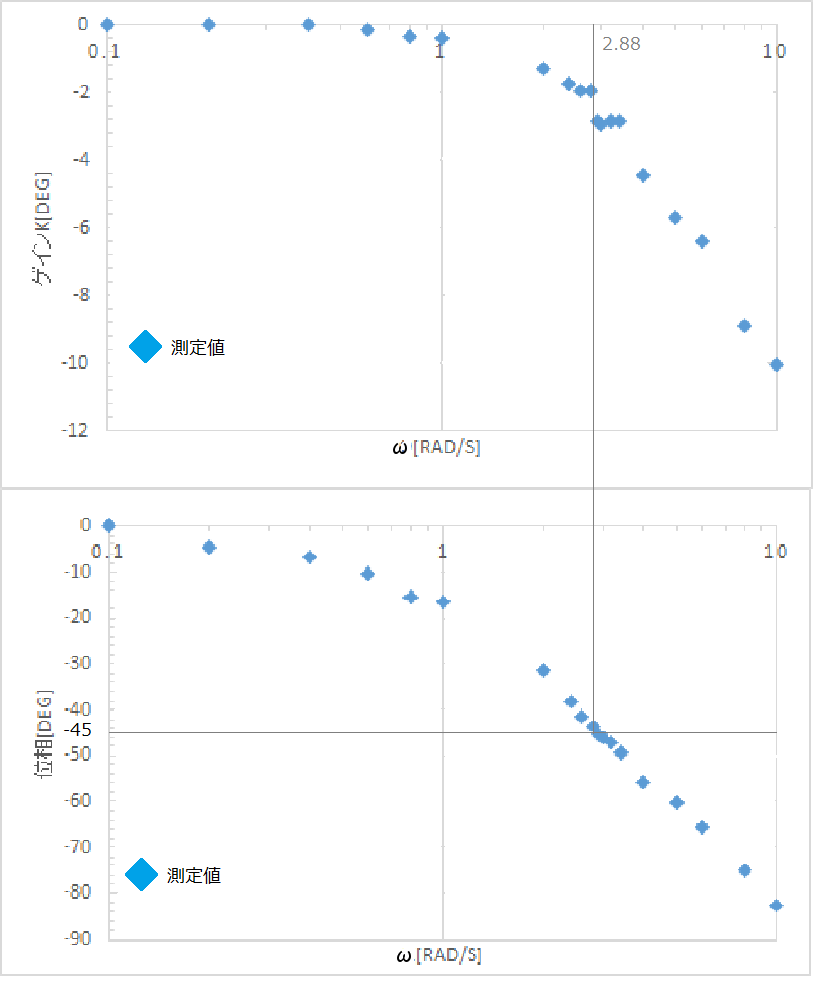
\includegraphics[scale=.7]{./picture/boardgraph.eps}
  \caption{ボード線図}
  \label{fig:board}
 \end{center}
\end{figure}

\newpage

 \section{考察}
 ボード線図より低周波ゲイン$\bar{k} = 0$なのでゲイン{\it k}は
 \begin{eqnarray*}
 \bar{k} & = &20\log{10}k \\
  0 & = & 20\log{10}k \\
  k & = & 1
 \end{eqnarray*}
 である.また位相$\phi_i = -45^\circ $のとき,折点周波数$\omega_d = 2.88$[rad/s].\\
 これより時定数{\it T}は
\begin{eqnarray*}
 \omega_d & = & \frac{1}{T} \\
 T & = & \frac{1}{2.88} \simeq 0.347
\end{eqnarray*}
である. \\
式\ref{eq5}の{\it k}と{\it T}にそれぞれ$k = 1$と$T = 0.347$を代入して得た位相とゲインを表\ref{tab:table2}に示す.これよりボード線図をプロットし,実験で得られたボード線図と比較する.結果を図\ref{fig:board2}に示す.

\begin{table}[h]
 \begin{center}
  \caption{一次遅れ系の同定結果}
  \begin{tabular}{|c|c|c|} \hline
   目標角度周波数 & ゲイン{\it k}[dB] & 位相$\phi_i$[deg]\\ \hline \hline
   0.1 & -0.01 & -1.99 \\ \hline
   0.2 & -0.02 & -3.97 \\ \hline
   0.3 & -0.05 & -5.95 \\ \hline
   0.4 & -0.83 & -7.91 \\ \hline
   0.5 & -0.13 & -9.85 \\ \hline
   0.6 & -0.18 & -11.8 \\ \hline
   0.7 & -0.25 & -13.7 \\ \hline
   0.8 & -0.32 & -15.5 \\ \hline
   0.9 & -0.40 & -17.4 \\ \hline
   1.0 & -0.49 & -19.2 \\ \hline
   2.0 & -1.71 & -34.8 \\ \hline
   3.0 & -3.19 & -46.2 \\ \hline
   4.0 & -4.67 & -54.3 \\ \hline
   5.0 & -6.04 & -60.1 \\ \hline
   6.0 & -7.28 & -64.4 \\ \hline
   7.0 & -8.39 & -67.7 \\ \hline
   8.0 & -9.40 & -70.2 \\ \hline
   9.0 & -10.3 & -72.3 \\ \hline
   10.0 & -11.2 & -74.0 \\ \hline
  \end{tabular}
  \label{tab:table2}
 \end{center}
\end{table}

\begin{figure}[htbp]
 \begin{center}
  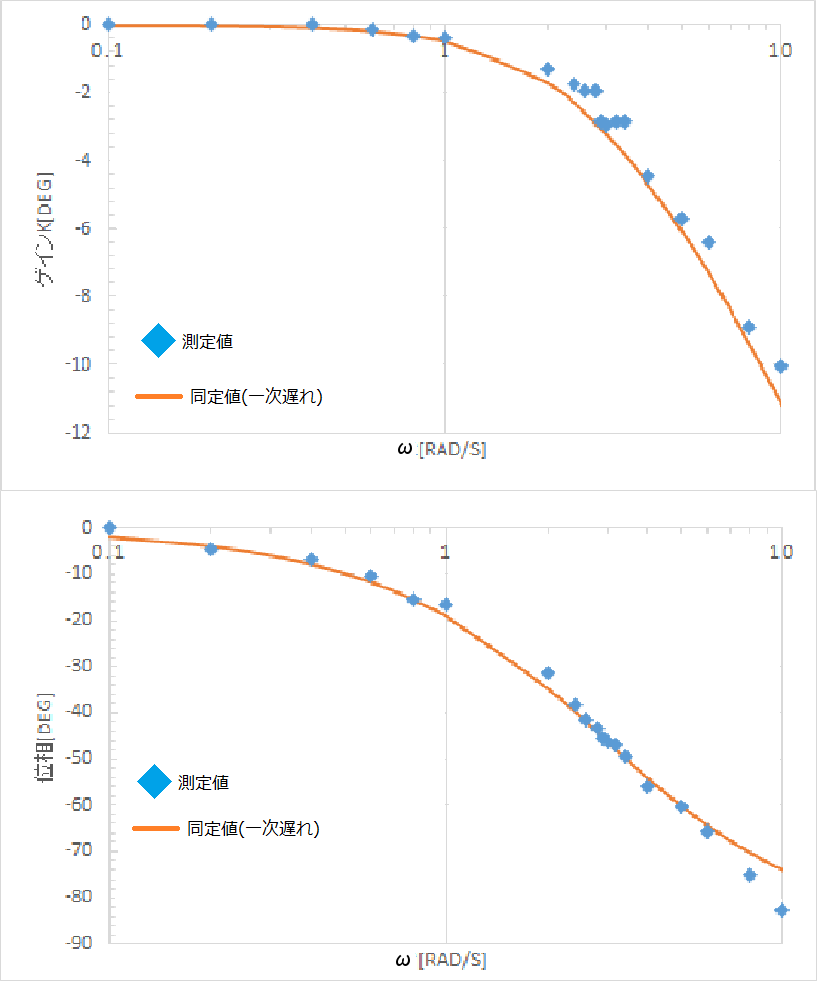
\includegraphics[scale=.7]{./picture/boardgraph2.eps}
  \caption{実験結果と同定値のボード線図}
  \label{fig:board2}
 \end{center}
\end{figure}

このとき,位相とゲインの両方について,低周波域ではグラフに差はほとんど見られないが,高周波になるほど差が大きくなっている.これは伝達関数を求める際,式\ref{eq3}のように近似したため,高周波になるほどこの近似との差が大きくなったためだと考える.近似を行わなかった場合,数学モデルは
\begin{equation}
\Phi(s) = \frac{f_a k_a k}{T T_a s^2 + T(f_a f_b + 1)s + f_a k_a} U(s)
 \label{eq14} 
\end{equation}
となる.これは2次遅れ系のモデルであり,式\ref{eq14}を$\Phi(s) = \frac{K}{(T_1 s + 1)(T_2 s + 1)} U(s)$とすると伝達関数は
\begin{equation}
G(j\omega) = K\{\frac{1 - T_1 T_2 \omega^2}{(1+(T_1 \omega)^2)(1 + (T_2 \omega)^2)} - j \frac{(T_1 + T_2)\omega}{(1+(T_1 \omega)^2)(1 + (T_2 \omega)^2)}\}
\label{eq16}
\end{equation}
となる.式\ref{eq16}より位相とゲインを求めると,

\begin{eqnarray}
 20 \log{10}|G(j\omega)| & = & 20 \log{10}\frac{K}{\sqrt{(1 + (T_1 \omega)^2)(1 + (T_2 \omega)^2)}} \nonumber \\ 
 \angle G(j \omega) & = & -\tan^{-1} \frac{(T_1 + T_2)\omega}{1 - T_1 T_2 \omega^2}
  \label{eq17}
\end{eqnarray}
式\ref{eq17}より,$\omega$[rad/s]の値が大きくなると式\ref{eq3}の近似による誤差の影響が無視できなくなる.




 \section{課題}
  \subsection{式\ref{eq6}の証明}
  入力電圧$u(t) = asin\omega_i t$をラプラス変換すると$U(s) = \frac{a\omega_i}{s^2 + \omega_i^2}$なので,式\ref{eq5}より
  \begin{eqnarray}
   \Theta(s) & = & \frac{k}{Ts + 1} \, \frac{\omega_i}{s^2 + \omega_i^2} \nonumber \\ & = & \frac{ak}{T}\,\frac{\omega_i}{(s+\frac{1}{T})(s^2 + \omega_i^2)}
    \label{eq7}
  \end{eqnarray}
  右辺について,部分分数分解をすると,
  \begin{eqnarray*}
   \frac{\omega_i}{(s+\frac{1}{T})(s^2 + \omega_i^2)} & =  & \frac{b_1}{s + \frac{1}{T}} + \frac{b_2 s}{s^2 + \omega_i^2} + \frac{b_3}{s^2 + \omega_i^2} \\ & = & b_1 \, \frac{1}{s + \frac{1}{T}} + b_2 \, \frac{s}{s^2 + \omega_i^2} + \frac{b_3}{\omega_i} \, \frac{\omega_i}{s^2 + \omega_i^2}
  \end{eqnarray*}
  これより,式\ref{eq7}の両辺を逆ラプラス変換して
  \begin{eqnarray*}
   \theta(t) & = & \frac{ak}{T} \, \{b_1 e^{-\frac{1}{T} t} + b_2 cos\omega_i t + b_3 sin\omega_i t \} \\ & = & b_i e^{-\frac{1}{T} t} + c_i \sin(\omega_i t + \phi_i)
  \end{eqnarray*}
  ただし,$\phi_i = \tan^{-1} \frac{b_3}{b_2}$である. \\
  したがって,式\ref{eq6}は成り立つ.

\newpage  

\thispagestyle{fancy}
\rhead{再1}

  \subsection{同定精度の向上}
  表\ref{tab:table1}の位相とゲインは伝達特性を式\ref{eq5}として式\ref{eq8}から求めた.これは伝達特性を一次遅れ系としたものであるが,式\ref{eq14}のように実際には二次遅れ系である.そこで,式\ref{eq17}より$T_1,T_2$を求めて同定精度の向上を行う. \\
表\ref{tab:table1}より$\omega  = 0.6 , 10.0$[rad/s]のとき位相$\phi_i = -10.4,-82.6$なので,
\begin{eqnarray*}
 T_1 = 0.045\\ 
 T_2 = 0.260
\end{eqnarray*}
また,$\omega = 0$のとき$20\log{10} |G(j\omega)| = 0$なので,式\ref{eq8}よりゲイン$K = 1$である.
これを式\ref{eq17}に代入してそれぞれのゲインと位相を求め,ボード線図をプロットする.結果を表\ref{table3},図\ref{fig:board3}に示す.
  
\begin{table}[h]
 \begin{center}
  \caption{二次遅れ系の同定結果}
  \begin{tabular}{|c|c|c|} \hline
   目標角度周波数 & ゲイン{\it k}[dB] & 位相$\phi_i$[deg]\\ \hline \hline
   0.1 & -0.01 & -1.74 \\ \hline
   0.2 & -0.05 & -3.49 \\ \hline
   0.3 & -0.10 & -5.22 \\ \hline
   0.4 & -0.18 & -6.95 \\ \hline
   0.5 & -0.26 & -8.67 \\ \hline
   0.6 & -0.39 & -10.4 \\ \hline
   0.7 & -0.53 & -12.1 \\ \hline
   0.8 & -0.67 & -13.7 \\ \hline
   0.9 & -0.84 & -15.4 \\ \hline
   1.0 & -1.01 & -17.0 \\ \hline
   2.0 & -3.13 & -32.0 \\ \hline
   3.0 & -5.31 & -44.0 \\ \hline
   4.0 & -7.26 & -53.4 \\ \hline
   5.0 & -8.96 & -60.8 \\ \hline
   6.0 & -10.5 & -66.8 \\ \hline
   7.0 & -11.8 & -71.7 \\ \hline
   8.0 & -12.9 & -75.9 \\ \hline
   9.0 & -14.1 & -79.4 \\ \hline
   10.0 & -15.1 & -82.6 \\ \hline
  \end{tabular}
  \label{table3}
 \end{center}
\end{table}

\newpage
\thispagestyle{fancy}
\rhead{再2}

\begin{figure}[htbp]
 \begin{center}
  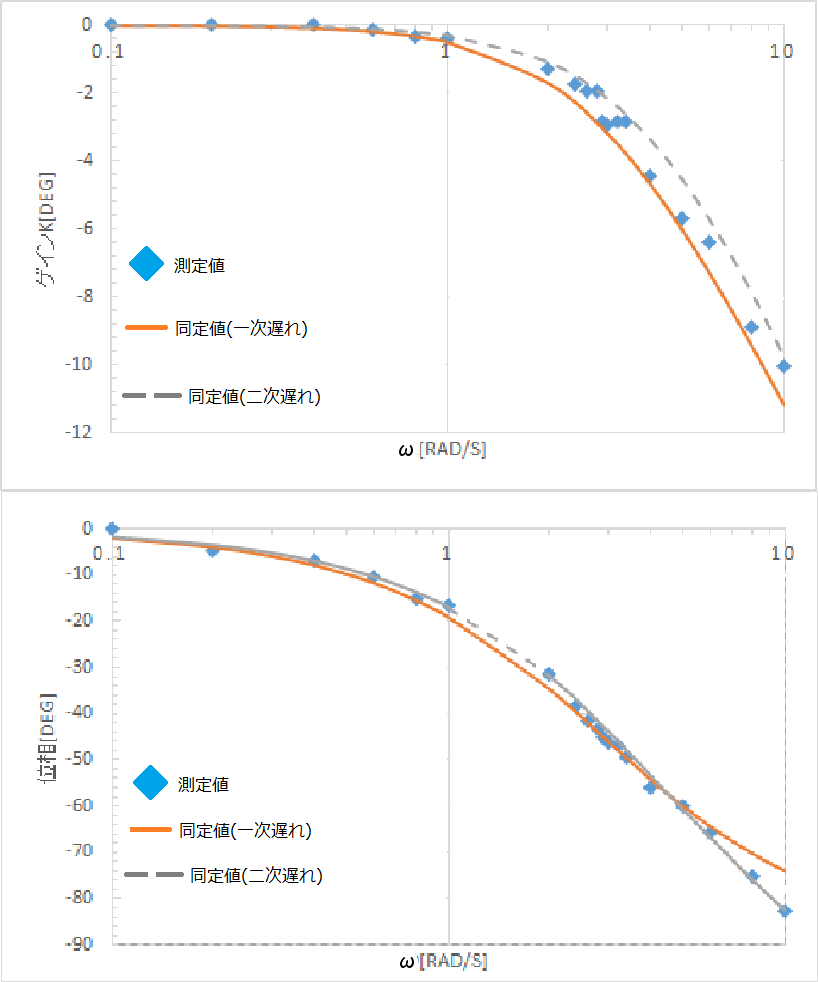
\includegraphics[scale=.7]{./picture/boardgraph3.eps}
  \caption{実験結果と同定値のボード線図}
  \label{fig:board3}
 \end{center}
\end{figure}

図\ref{fig:board3}よりモデルを二次遅れ系として同定を行った場合,一次遅れ系とした時より同定精度が向上していることがわかる.


\section{まとめ}
サーボモータを対象として,制御対象の未知パラメータを同定する方法の一つを習得出来た.また,同定において精度を向上させるためには対象をできるだけ正確にモデル化することが重要である.
 
\newpage

\thispagestyle{fancy}
\rhead{再々1}



\section{同定精度の向上についての補足}
一次遅れ系と二次遅れ系のゲインと位相について測定値との相対誤差を求める.図\ref{fig:board3}より特に誤差の大きい$\omega \geq 5$について考える.表より,1次遅れ系より2次遅れ系で同定した時の方が同定精度が向上していることがわかる.

\begin{table}[hb]
 \begin{center}
  \caption{ゲインについての誤差}
  \begin{tabular}{|c||c||c|c||c|c|} \hline
   \multicolumn{1}{|c||}{$\omega$[rad/s]}
   & \multicolumn{1}{c||}{測定値}
       & \multicolumn{2}{|c||}{1次遅れ系}
   & \multicolumn{2}{|c|}{2次遅れ系} \\ \hline \hline
   - & ゲイン[dB] & ゲイン[dB] &  相対誤差[\%] & ゲイン[dB] & 相対誤差[\%] \\ \hline \hline
   5  & -5.68 & -6.04 & 6.27 & -4.51 & 20.6 \\ \hline
   6  & -6.38 & -7.28 & 14.1 & -5.66 & 11.3 \\ \hline
   8  & -8.87 & -9.40 & 5.97 & -7.78 & 12.3 \\ \hline
   10 & -10.0 & -11.2 & 11.5 & -9.68 & 3.22\\ \hline
  \end{tabular}
 \end{center}
\end{table}

\begin{table}[hb]
 \begin{center}
  \caption{位相についての誤差}
  \begin{tabular}{|c||c||c|c||c|c|} \hline
   \multicolumn{1}{|c||}{$\omega$[rad/s]}
   & \multicolumn{1}{c||}{測定値}
       & \multicolumn{2}{|c||}{1次遅れ系}
   & \multicolumn{2}{|c|}{2次遅れ系} \\ \hline \hline
   - & 位相[deg] & 位相[deg] &  相対誤差[\%] & 位相[deg] & 相対誤差[\%] \\ \hline \hline
   5  & -60.1 & -60.1 & 0.03 & -60.8 & 1.23 \\ \hline
   6  & -65.6 & -64.4 & 1.89 & -66.8 & 1.78 \\ \hline
   8  & -75.2 & -70.2 & 6.57 & -75.9 & 0.90 \\ \hline
   10 & -82.6 & -74.0 & 10.4 & -82.6 & $2.86*10^{-9}$\\ \hline
  \end{tabular}
 \end{center}
\end{table}


\end{document}
